\documentclass[12pt,a4paper]{article}

\usepackage[utf8]{inputenc}
\usepackage[T1]{fontenc}
\usepackage[spanish,es-tabla]{babel}
\usepackage{lmodern}
\usepackage[a4paper,margin=2.35cm]{geometry}
\usepackage{graphicx}
\usepackage{float}
\usepackage{array}
\usepackage{longtable}
\usepackage{booktabs}
\usepackage{enumitem}
\usepackage{ragged2e}
\usepackage{hyperref}
\usepackage{csquotes}
\usepackage[backend=biber,style=ieee,sorting=none]{biblatex}
\addbibresource{referencias.bib}
\hypersetup{hidelinks}
\setlength{\parindent}{0pt}
\setlength{\parskip}{5pt}
\setlength{\tabcolsep}{4pt}
\renewcommand{\arraystretch}{1.15}
\newcolumntype{L}[1]{>{\RaggedRight\arraybackslash}p{#1}}

\begin{document}

\begin{titlepage}
\centering
{\Large\textbf{Universidad Técnica Estatal de Quevedo}}\par\vspace{0.3cm}
{\large Facultad de Ciencias de la Computación}\par
{\large Carrera de Software}\par\vspace{1.0cm}
{\large\textbf{Ingeniería de Requisitos (ISR-401)}}\par\vspace{1.5cm}
{\LARGE\textbf{TA-TAR-01 -- SUM}}\par\vspace{0.3cm}
{\Large Trabajo individual: IEEE 29148 y tipos de requisitos de un sistema conocido}\par\vspace{1.0cm}
{\Large\textbf{Sistema de estudio: Steam}}\par\vfill
\begin{flushleft}
\textbf{Estudiante:} Luis Yepez\\
\textbf{Fecha límite indicada en el SGA:} 11 de noviembre de 2026, 23:59
\end{flushleft}
\end{titlepage}

\section{Resumen analítico de ISO/IEC/IEEE 29148:2018}

\subsection*{Qué es un requisito y por qué importa}

Cuando se quiere crear o mejorar un programa, lo primero es entender qué necesitan las personas que van a utilizarlo. La norma ISO/IEC/IEEE 29148:2018 ayuda a pasar de esas necesidades a requisitos claros, que después puedan revisarse y comprobarse \cite{iso29148,pohl2025}. Si una petición se escribe de forma muy general, el equipo puede entender algo diferente de lo que esperaba el usuario.

La cláusula 3.1.19 presenta el requisito como la expresión de una necesidad, con las condiciones y límites que le correspondan. Por ejemplo, decir que Steam debería descargar los juegos ``mejor'' no explica qué hay que cambiar. Puede tratarse de la velocidad, de recuperar una descarga interrumpida o de mostrar el avance con más claridad. Antes de establecer una solución, conviene descubrir qué problema existe de verdad.

En la cláusula 5.2.3 se explica cómo las necesidades se van transformando en requisitos. No basta con anotar lo primero que dice un usuario: hay que entender su situación, aclarar las dudas y definir qué espera del sistema. En Steam, la tienda, la biblioteca y el gestor de descargas permiten observar varias funciones. Esas pantallas ayudan a plantear requisitos, pero por sí solas no muestran cómo funciona toda la plataforma ni permiten conocer sus resultados de rendimiento o seguridad.

\subsection*{Cómo escribir un requisito bien formado}

La cláusula 5.2.4 se ocupa de cómo construir un requisito. La idea es decir con claridad qué debe hacer el sistema o qué condición debe cumplir, sin mezclar demasiadas cosas en una sola frase. También conviene dejar claro a qué parte del sistema se refiere. Por ejemplo, ``El cliente de Steam debe mostrar el porcentaje de avance de una descarga activa'' es más preciso que ``El usuario debe poder ver cómo va la descarga''.

No todos los requisitos necesitan números, pero sí deben poder comprobarse. Cuando se pide un tiempo máximo, un porcentaje o una cantidad, hay que explicar cómo se va a medir. Para este ejercicio se proponen cifras que sirven para practicar la redacción. No son mediciones realizadas en Steam ni valores confirmados por la empresa.

\subsection*{Características de un requisito individual}

La cláusula 5.2.5 explica qué hace que un requisito esté bien escrito. Debe ser \emph{necesario}, es decir, responder a algo que hace falta; \emph{apropiado}, con el detalle adecuado; e \emph{inequívoco}, para que no tenga dos significados distintos. También debe estar \emph{completo}, expresar una sola obligación y resultar posible de realizar. Por último, debe poder verificarse, describir correctamente la necesidad y seguir las reglas de redacción que se hayan definido.

Esto se entiende mejor con un ejemplo. Pedir que una descarga sea instantánea puede ser poco realista, porque depende de la conexión y del tamaño del juego. En cambio, pedir que una descarga interrumpida pueda reanudarse dentro de un tiempo definido permite preparar una prueba. De todas formas, antes de aprobar ese tiempo habría que comprobar que sea adecuado para los usuarios.

Palabras como ``rápido'', ``seguro'', ``fácil'' o ``siempre'' pueden servir en una conversación, pero generan dudas cuando quedan solas en un requisito. No se trata de palabras prohibidas en cualquier situación; el problema aparece cuando no se explica qué significan. Si se pide una búsqueda rápida, por ejemplo, debe quedar claro cuánto puede tardar, en qué condiciones se medirá y qué resultado se considera aceptable.

\subsection*{Calidad del conjunto de requisitos}

La cláusula 5.2.6 trata la calidad de todos los requisitos vistos en conjunto. Aunque cada uno esté bien redactado, el documento tendrá problemas si hay contradicciones o si falta alguna función importante. Un ejemplo sería pedir que el usuario pueda pausar una descarga y, al mismo tiempo, exigir que ninguna descarga pueda detenerse. Las dos instrucciones chocarían entre sí.

En un sistema como Steam hay que mirar varias partes relacionadas: buscar juegos, consultar la biblioteca, comprar, descargar e instalar. También se necesitan reglas para las compras, límites de compatibilidad y condiciones de calidad. El modelo ISO/IEC 25010:2023 sirve para ordenar las características de calidad, como seguridad, rendimiento y disponibilidad \cite{iso25010}. Revisar los requisitos de forma individual y en conjunto ayuda a descubrir errores antes de desarrollar o cambiar el sistema.

\clearpage
\section{Glosario de diez términos de la cláusula 3}

Estos diez términos pertenecen a la cláusula 3 de ISO/IEC/IEEE 29148:2018. Cada uno se explica con palabras sencillas y se acompaña de un ejemplo relacionado con Steam \cite{iso29148}.

\begin{enumerate}[leftmargin=*,itemsep=6pt]
\item \textbf{Requisito (3.1.19):} expresión precisa de una necesidad con condiciones asociadas. \textit{Ejemplo:} mostrar el progreso porcentual de la descarga activa.
\item \textbf{Elicitación de requisitos (3.1.20):} obtención organizada de necesidades de los interesados. \textit{Ejemplo:} preguntar a jugadores qué información necesitan para gestionar descargas.
\item \textbf{Ingeniería de Requisitos (3.1.21):} disciplina que desarrolla, analiza, documenta y gestiona los requisitos. \textit{Ejemplo:} revisar conjuntamente las necesidades de la tienda, la biblioteca y las descargas.
\item \textbf{Gestión de requisitos (3.1.22):} mantenimiento y seguimiento de los requisitos durante el proyecto. \textit{Ejemplo:} registrar el cambio de criterio para reanudar una descarga interrumpida.
\item \textbf{Trazabilidad (3.1.23):} relación documentada de un requisito con su origen y elementos derivados. \textit{Ejemplo:} vincular el requisito de pausar descargas con la captura del gestor y su prueba de aceptación.
\item \textbf{Matriz de trazabilidad (3.1.24):} registro organizado de esas relaciones. \textit{Ejemplo:} una tabla que una RF-04 con la evidencia 3 y el caso de prueba correspondiente.
\item \textbf{Validación de requisitos (3.1.25):} evaluación de si los requisitos representan las necesidades correctas de los interesados. \textit{Ejemplo:} confirmar con jugadores que necesitan pausar descargas sin perder progreso.
\item \textbf{Verificación de requisitos (3.1.26):} revisión de si los requisitos están bien formulados. \textit{Ejemplo:} comprobar que RC-01 indica operación, métrica, unidad, umbral y contexto.
\item \textbf{Especificación de requisitos de software (3.1.27):} conjunto estructurado de requisitos del software y sus interfaces. \textit{Ejemplo:} el documento con requisitos de búsqueda, biblioteca y descargas del cliente.
\item \textbf{Parte interesada (3.1.28):} persona u organización que tiene intereses relacionados con el sistema. \textit{Ejemplo:} jugadores que utilizan Steam y responsables de mantener la plataforma.
\end{enumerate}

\section{Sistema seleccionado y evidencias}

Steam se analiza como plataforma de distribución y gestión de videojuegos. Las tres capturas propias aportadas para el ejercicio corresponden a la \textbf{biblioteca}, la \textbf{tienda} y el \textbf{gestor de descargas}. Sirven para reconocer funciones visibles, pero no certifican tiempos de respuesta, niveles de disponibilidad, medidas de seguridad ni reglas internas de la plataforma.

\begin{figure}[H]
\centering

\includegraphics[width=0.91\textwidth]{evidencias/captura1.png}
\caption{Captura propia: biblioteca de videojuegos de Steam.}
\label{fig:biblioteca}
\end{figure}

\begin{figure}[H]
\centering

\includegraphics[width=0.91\textwidth]{evidencias/captura2.png}
\caption{Captura propia: tienda de Steam y juegos destacados.}
\label{fig:tienda}
\end{figure}

\begin{figure}[H]
\centering
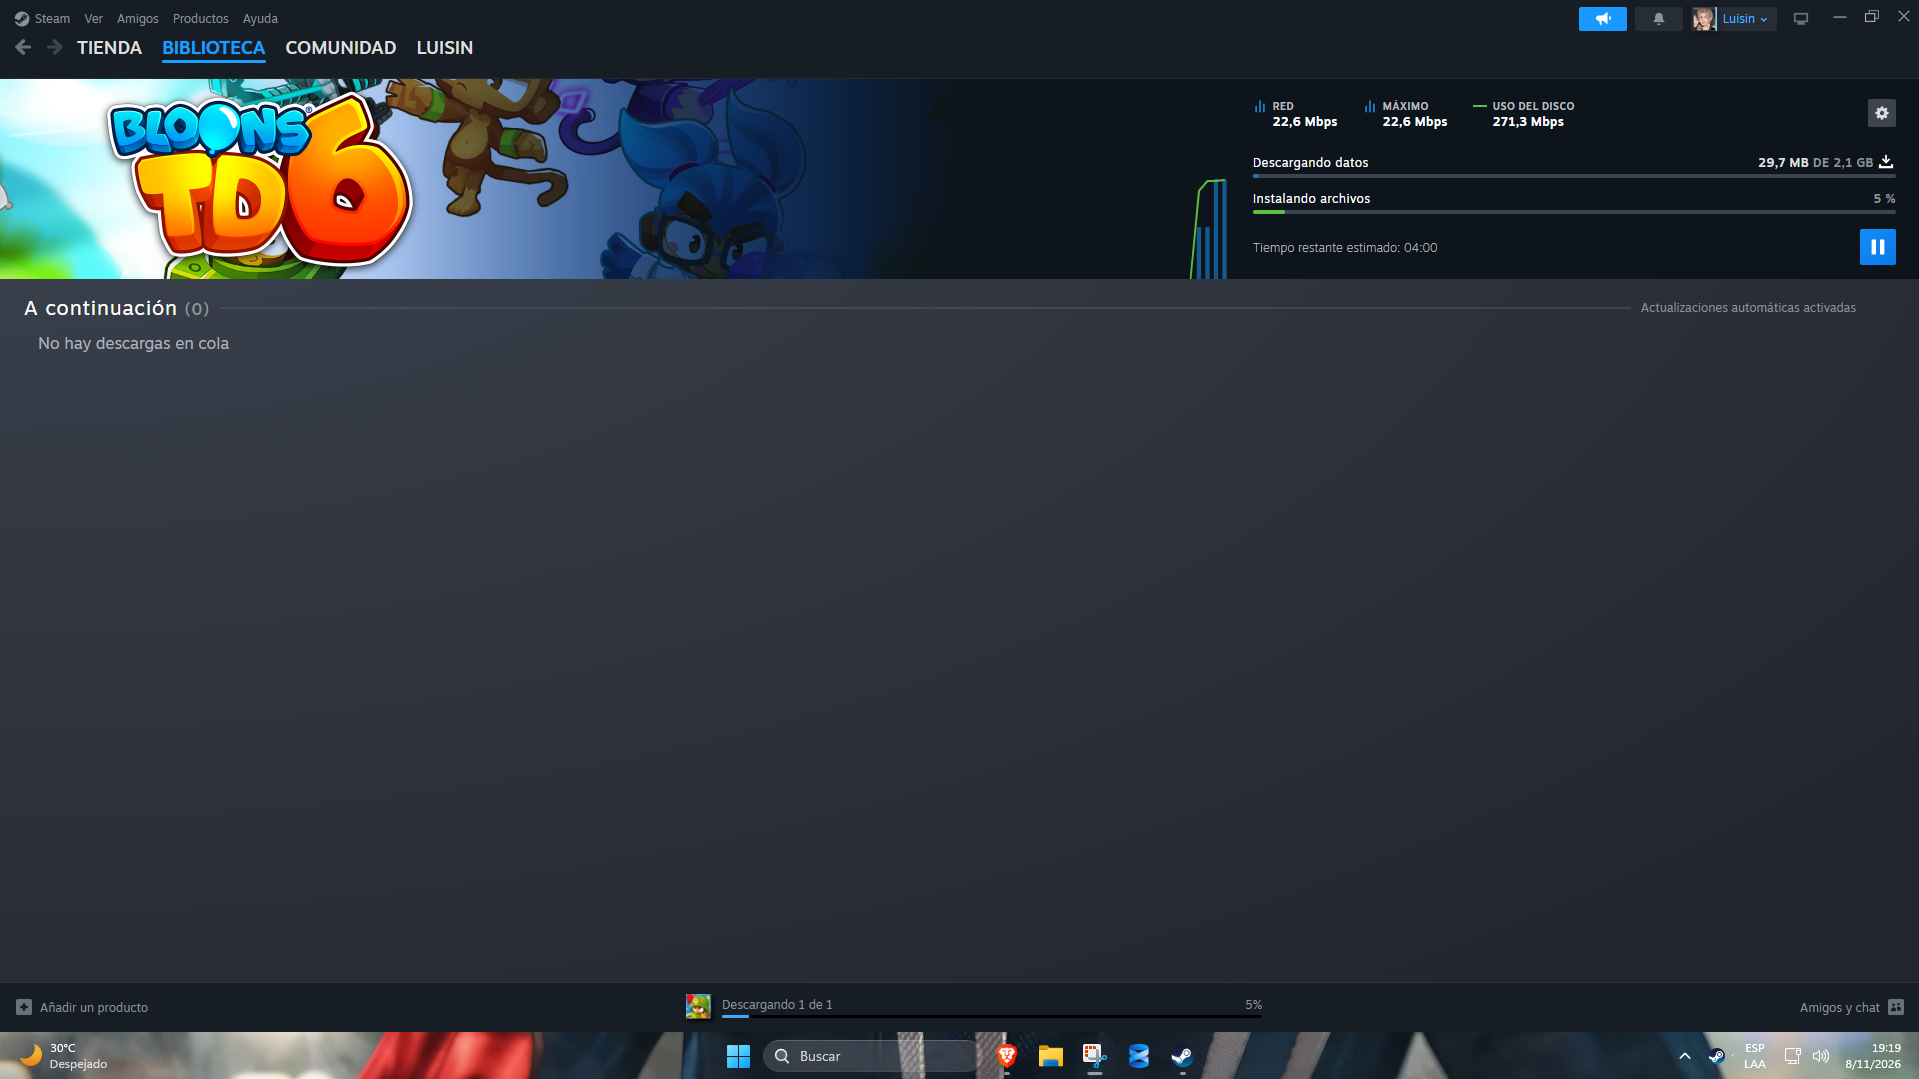
\includegraphics[width=0.91\textwidth]{evidencias/captura3.png}
\caption{Captura propia: progreso de una descarga.}
\label{fig:descargas}
\end{figure}

\section{Formulación de quince requisitos propuestos}

Los quince requisitos se distribuyen en \textbf{cinco tipos}: funcionales (4), calidad (5), interfaz (2), reglas de negocio o dominio (2) y restricciones (2). Son formulaciones \textbf{propuestas para el ejercicio}, no afirmaciones de cumplimiento real. Las características de calidad se organizan según ISO/IEC 25010:2023 \cite{iso25010}.

\subsection{Funcionales (4)}
\begin{description}[leftmargin=!,labelwidth=1.5cm]
\item[RF-01.] El cliente deberá permitir buscar juegos por una palabra del título y mostrar los resultados coincidentes en la tienda.
\item[RF-02.] El cliente deberá permitir agregar un juego a la lista de deseados y retirarlo de esa lista.
\item[RF-03.] El cliente deberá mostrar al usuario autenticado los videojuegos asociados a su biblioteca.
\item[RF-04.] El cliente deberá permitir pausar y reanudar la descarga de un videojuego desde el gestor de descargas.
\end{description}

\subsection{De calidad (5)}
\begin{description}[leftmargin=!,labelwidth=1.5cm]
\item[RC-01.] \textbf{Eficiencia del desempeño: comportamiento temporal.} En una prueba con 150 búsquedas simultáneas, al menos el 95\% de las solicitudes deberá mostrar resultados en 2 segundos o menos. \textbf{Métrica:} tiempo de respuesta; \textbf{unidad:} segundos; \textbf{umbral:} percentil 95 $\leq 2$ s.
\item[RC-02.] \textbf{Fiabilidad: recuperabilidad.} Tras restablecerse la conexión durante una descarga interrumpida, el cliente deberá permitir reanudarla en un máximo de 30 segundos sin reiniciar la descarga completa. \textbf{Métrica:} tiempo hasta reanudación; \textbf{unidad:} segundos; \textbf{umbral:} $\leq 30$ s.
\item[RC-03.] \textbf{Seguridad: confidencialidad.} El sistema deberá rechazar el 100\% de 100 solicitudes de prueba realizadas sin autorización para consultar información privada de otra cuenta. \textbf{Métrica:} accesos indebidos rechazados; \textbf{unidad:} porcentaje; \textbf{umbral:} 100\%.
\item[RC-04.] \textbf{Capacidad de interacción: facilidad de aprendizaje.} En una prueba con 20 personas que no hayan utilizado el cliente, al menos 18 deberán localizar un juego de la biblioteca en un máximo de 60 segundos sin ayuda. \textbf{Métrica:} participantes que completan la tarea; \textbf{unidad:} personas y segundos; \textbf{umbral:} 18/20 en $\leq 60$ s.
\item[RC-05.] \textbf{Fiabilidad: disponibilidad.} El servicio de consulta de la tienda deberá alcanzar una disponibilidad mínima del 99,5\% durante 30 días consecutivos. \textbf{Métrica:} tiempo operativo / tiempo total; \textbf{unidad:} porcentaje; \textbf{umbral:} $\geq 99,5\%$.
\end{description}

\subsection{De interfaz (2)}
\begin{description}[leftmargin=!,labelwidth=1.5cm]
\item[RI-01.] La pantalla de descargas deberá mostrar, para cada descarga activa, porcentaje de avance, tamaño recibido y velocidad de transferencia.
\item[RI-02.] Al seleccionar un videojuego de la biblioteca, el cliente deberá abrir una vista de detalle con la opción de instalarlo o iniciarlo, según su estado local.
\end{description}

\subsection{Reglas de dominio o negocio (2)}
\begin{description}[leftmargin=!,labelwidth=1.5cm]
\item[RD-01.] Cuando una compra de una licencia de juego resulte confirmada, el título deberá quedar asociado a la biblioteca de la cuenta compradora, salvo que las condiciones del producto indiquen un tipo de acceso diferente.
\item[RD-02.] Si una oferta tiene fecha de inicio y finalización, el descuento deberá aplicarse únicamente a compras confirmadas dentro de su periodo de vigencia, según la hora de referencia definida para la tienda.
\end{description}

\subsection{Restricciones (2)}
\begin{description}[leftmargin=!,labelwidth=1.5cm]
\item[RT-01.] La versión de cliente considerada en este ejercicio deberá ser compatible con Windows 11 de 64 bits.
\item[RT-02.] Las pantallas principales del cliente consideradas en este ejercicio deberán ofrecer textos de navegación en español.
\end{description}

\section{Tabla de clasificación y criterios de aceptación}

\small
\begin{longtable}{L{1.3cm}L{2.8cm}L{9.4cm}}
\caption{Criterios de aceptación propuestos para los quince requisitos.}\label{tab:criterios}\\
\toprule
\textbf{ID} & \textbf{Tipo} & \textbf{Criterio de aceptación comprobable}\\
\midrule\endfirsthead
\toprule\textbf{ID} & \textbf{Tipo} & \textbf{Criterio de aceptación comprobable}\\
\midrule\endhead
RF-01 & Funcional & Al introducir una palabra de un título existente, la tienda presenta resultados que la contienen.\\
RF-02 & Funcional & Tras agregar y retirar un juego, la lista de deseados refleja ambos cambios.\\
RF-03 & Funcional & Una cuenta autenticada puede ver en su biblioteca los juegos asociados a ella en el escenario de prueba.\\
RF-04 & Funcional & Al pulsar Pausar, la descarga se detiene; al pulsar Reanudar, continúa desde el avance guardado.\\
RC-01 & Calidad: tiempo & En 150 solicitudes concurrentes de prueba, al menos el 95\% responde en $\leq 2$ segundos.\\
RC-02 & Calidad: recuperación & Tras restaurar la red, la descarga puede reanudarse en $\leq 30$ segundos sin volver a descargar desde cero.\\
RC-03 & Calidad: seguridad & Se rechazan 100 de 100 accesos de prueba sin autorización a datos privados de otra cuenta.\\
RC-04 & Calidad: interacción & Al menos 18 de 20 participantes nuevos encuentran un juego en su biblioteca en $\leq 60$ segundos.\\
RC-05 & Calidad: disponibilidad & Las mediciones de 30 días arrojan disponibilidad de la tienda $\geq 99,5\%$.\\
RI-01 & Interfaz & Con una descarga activa se muestran porcentaje, tamaño recibido y velocidad de transferencia.\\
RI-02 & Interfaz & La vista del juego presenta Instalar si no está instalado e Iniciar si está listo para jugar.\\
RD-01 & Regla de negocio & Una compra de prueba confirmada incorpora el título a la biblioteca de la cuenta, salvo la excepción de acceso declarada.\\
RD-02 & Regla de negocio & Una compra de prueba dentro de la vigencia aplica el descuento y otra fuera de ella no lo aplica.\\
RT-01 & Restricción & El cliente previsto para el ejercicio inicia y permite navegar en Windows 11 de 64 bits.\\
RT-02 & Restricción & Tienda, biblioteca y gestor de descargas muestran sus textos principales en español.\\
\bottomrule
\end{longtable}
\normalsize

\section{Autoevaluación y versión corregida de cada requisito}

La revisión siguiente aplica claridad, singularidad, completitud y verificabilidad como criterios orientativos de la cláusula 5.2.5 \cite{iso29148}. En cada caso se muestra una frase poco clara, se explica su problema y se presenta una forma más precisa de escribirla. Estas correcciones son parte del ejercicio y no representan pruebas ejecutadas en Steam.
\\\\
\begin{enumerate}[leftmargin=*,itemsep=8pt]
\item \textbf {RF-01.} Inicial: ``Steam debe buscar juegos''. \\ \textbf{Problema:} no indica el criterio de búsqueda. \\ \textbf{Corregida:} El cliente deberá permitir buscar juegos por una palabra del título y mostrar las coincidencias en la tienda.
\item \textbf{RF-02.} Inicial: ``Gestionar favoritos''. \\\textbf{Problema:} se desconoce qué operaciones incluye. \\ \textbf{Corregida:} El cliente deberá permitir agregar un juego a la lista de deseados y retirarlo de esa lista.
\item \textbf{RF-03.} Inicial: ``Mostrar juegos''. \\\textbf{Problema:} no identifica la colección ni el usuario. \\\textbf{Corregida:} El cliente deberá mostrar al usuario autenticado los videojuegos asociados a su biblioteca.
\item \textbf{RF-04.} Inicial: ``Controlar descargas''.\\ \textbf{Problema:} el verbo es general. \\ \textbf{Corregida:} El cliente deberá permitir pausar y reanudar la descarga de un videojuego desde el gestor de descargas.
\item \textbf{RC-01.} Inicial: ``La búsqueda debe ser rápida''. \\\textbf{Problema:} no es verificable. \\\textbf{Corregida:} Al menos el 95\% de 150 búsquedas concurrentes deberá responder en 2 segundos o menos.
\item \textbf{RC-02.} Inicial: ``Las descargas no deben fallar''. \\\textbf{Problema:} plantea una condición absoluta. \\\textbf{Corregida:} Tras recuperar la conexión, la descarga deberá poder reanudarse en 30 segundos o menos sin reiniciarse desde cero.
\item \textbf{RC-03.} Inicial: ``Las cuentas deben ser seguras''. \\\textbf{Problema:} no concreta qué proteger. \\\textbf{Corregida:} Se deberán rechazar las 100 solicitudes de una prueba de acceso sin autorización a datos privados de otra cuenta.
\item \textbf{RC-04.} Inicial: ``La biblioteca debe ser fácil''. \\\textbf{Problema:} no define usuarios ni tarea. \\\textbf{Corregida:} Al menos 18 de 20 personas nuevas deberán encontrar un juego de su biblioteca en 60 segundos o menos sin ayuda.
\item \textbf{RC-05.} Inicial: ``La tienda siempre funcionará''. \\\textbf{Problema:} ``siempre'' impide medir cumplimiento realista.\\ \textbf{Corregida:} El servicio de consulta de la tienda deberá mantener disponibilidad de al menos 99,5\% durante 30 días consecutivos.
\item \textbf{RI-01.} Inicial: ``Mostrar la descarga''.\\ \textbf{Problema:} faltan elementos de la interfaz. \\\textbf{Corregida:} La pantalla de descargas deberá mostrar porcentaje, tamaño recibido y velocidad de transferencia de la descarga activa.
\\\\
\item \textbf{RI-02.} Inicial: ``Abrir los juegos''. \\\textbf{Problema:} no describe la respuesta ante una selección. \\\textbf{Corregida:} Al seleccionar un juego de la biblioteca, deberá aparecer una vista de detalle con Instalar o Iniciar según su estado.
\item \textbf{RD-01.} Inicial: ``Los juegos comprados son del usuario''. \\\textbf{Problema:} no aclara el registro de la licencia ni sus excepciones. \\\textbf{Corregida:} Tras confirmarse la compra de una licencia, el juego se asociará a la cuenta compradora, salvo condiciones de acceso distintas declaradas para el producto.
\item \textbf{RD-02.} Inicial: ``Aplicar ofertas correctamente''.\\ \textbf{Problema:} falta una condición temporal. \\\textbf{Corregida:} Los descuentos se aplicarán únicamente a las compras confirmadas durante el periodo de vigencia de la oferta, de acuerdo con la hora de referencia de la tienda.
\item \textbf{RT-01.} Inicial: ``Funcionar en PC''. \\\textbf{Problema:} no identifica el entorno. \\\textbf{Corregida:} La versión de cliente considerada deberá ser compatible con Windows 11 de 64 bits.
\item \textbf{RT-02.} Inicial: ``Estar en nuestro idioma''. \\\textbf{Problema:} es ambiguo. \\\textbf{Corregida:} Las pantallas principales de tienda, biblioteca y descargas deberán presentar sus textos de navegación en español.
\end{enumerate}

\section{Reflexión personal}

Elegí Steam porque es una aplicación que conozco y utilizo para ver mis juegos y gestionar descargas. Cuando revisé las capturas de la biblioteca, la tienda y el apartado de descargas, noté que detrás de cada opción hay varias cosas que el programa debe hacer bien. Por ejemplo, no basta con mostrar un botón para pausar una descarga; también importa que el avance se conserve y que el usuario pueda continuarla después.

Al escribir los requisitos me di cuenta de que algunas frases que usamos normalmente no son suficientes. Decir que algo debe funcionar ``rápido'' parece claro hasta que alguien pregunta cuántos segundos son aceptables. Lo mismo ocurre con la seguridad o con la facilidad de uso. Por eso fue necesario indicar acciones concretas y, en los requisitos de calidad, proponer formas de medir los resultados.

También entendí que los requisitos tienen que llevarse bien entre sí. La tienda, la biblioteca y las descargas son partes distintas, pero una acción puede afectar a otra. Si una compra se confirma, por ejemplo, el juego debe quedar disponible en la biblioteca según sus condiciones de acceso. Esta actividad me ayudó a mirar una aplicación que uso con frecuencia de una manera más detallada y a entender por qué es importante escribir requisitos claros antes de desarrollar software.

\section{Herramientas utilizadas}

Para organizar el archivo LaTeX y trabajar propuestas de redacción, requisitos y tablas se utilizó ChatGPT de OpenAI (GPT-6) como apoyo. Se consultó la terminología de ISO/IEC/IEEE 29148:2018 para comprobar las referencias a las cláusulas citadas. Las tres imágenes son capturas de Steam proporcionadas para esta actividad. Los valores de tiempo, porcentajes y otras medidas del ejercicio son propuestas, no resultados de pruebas realizadas sobre Steam.

\printbibliography[heading=bibintoc,title={Referencias bibliográficas}]
\end{document}
